Les raisonnements probabilistes en \textbf{Intelligence Artificielle} sont basés sur la théorie 
des probabilités et permettent de modéliser des situations 
où l'on ne peut pas prédire avec certitude le résultat d'une action (\textit{environnements non-déterministes}).

\subsection{Quelques définitions} % (fold)
\label{sub:quelques_definitions}


\begin{definition}{Événement élémentaire}{evenementelementaire}
    Un état possible de l'environnement. 
    Il est souvent noté $\omega$.
\end{definition}

\begin{definition}{Univers}{univers}
    L'ensemble de tous les événements élémentaires possible.
    Il est souvent noté $\Omega$.
\end{definition}

\begin{definition}{Variable aléatoire}{varaleatoire}
    Une \textbf{variable aléatoire} est une fonction qui associe à chaque événement élémentaire 
    d'un espace probabilisé un nombre réel. 
    On note $A$ une variable aléatoire et $\omega$ une valeur prise par $A$. 
    On note $P(A=\omega)$ la probabilité que $A$ prenne la valeur $\omega$. 
    On note $P(A)$ la loi de probabilité de $A$. 
\end{definition}

\begin{remark}\leavevmode
    C'est une manière de quantifier de numériquement les résultats d'une expérience aléatoire.

    Fonction qui prend en entrée un événement élémentaire et qui renvoie un nombre réel (quantification).
\end{remark}

% subsection Quelques definitions (end)

\subsection{Rappel proba} % (fold)
\label{sub:rappel_proba}

\begin{definition}{Probabilité Conjointes}{probconj}
    La probabilité conjointe de deux variables aléatoires $A$ et $B$ est la probabilité de l'événement 
    où $A$ prend la valeur $x$ \textbf{ET} $B$ prend la valeur $y$.
    \begin{align*}
        P(A=x , B=y) &= P(A=x \cap B=y) \\ 
                    &= P(A=x | B=y)P(B=y) \\ 
                    &= P(B=y | A=x)P(A=x)
    \end{align*}
\end{definition}

\begin{figure}[H]
    \begin{center}
        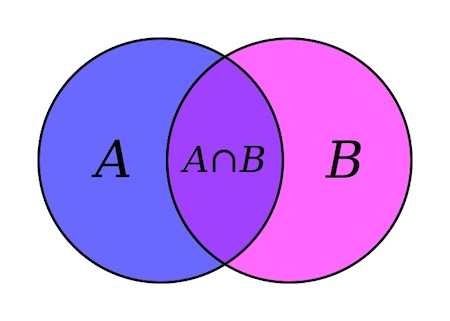
\includegraphics[width=0.3\textwidth]{pictures/conjproba.jpg}
    \end{center}
    \caption{Diagramme de Venn de $P(A \cap B)$}\label{fig:conjproba}
\end{figure}


% \begin{example}\leavevmode
%     Rajouter des exs ?
% \end{example}

\begin{definition}{Probabilité d'une disjonction}{probdisonction}
    La probabilité d'une disjonction de deux variables aléatoires $A$ et $B$ est la probabilité de l'événement 
    où $A$ prend la valeur $x$ \textbf{OU} $B$ prend la valeur $y$.
    \begin{equation}
        P(A=x \cup B=y) = P(A=x) + P(B=y) - P(A=x\cap B=y)
    \end{equation}
    La sousstraction est nécessaire pour éviter de compter deux fois la probabilité de l'intersection.
\end{definition}

\begin{figure}[H]
    \begin{center}
        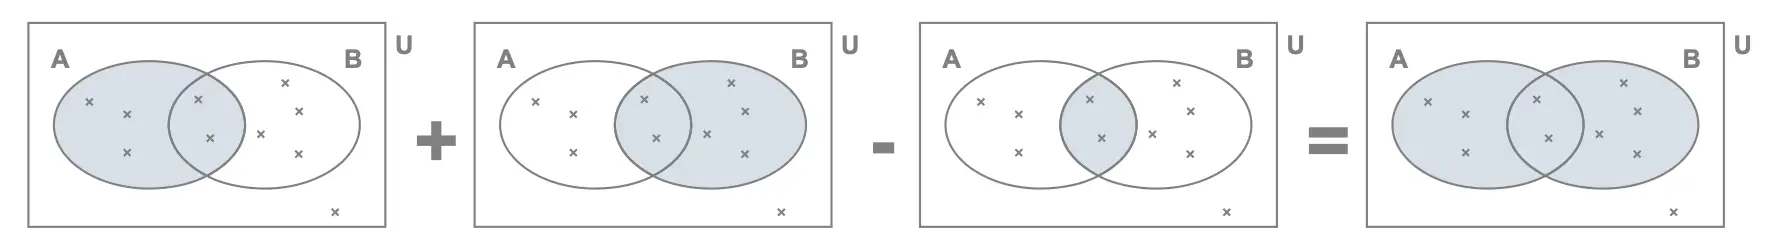
\includegraphics[width=0.95\textwidth]{pictures/disjproba.png}
    \end{center}
    \caption{Diagramme de Venn de $P(A \cup B)$}\label{fig:disjproba}
\end{figure}


% \newpage


\begin{definition}{Probabilité Marginale}{probmarginale}
    La probabilité marginale d'une variable aléatoire $A$ est la probabilité de l'événement 
    où $A$ prend la valeur $x$.
    \begin{equation}
        P(A=x) = \sum_{y \in B} P(A=x \cap B=y)
    \end{equation} 
    Où $B$ prend toutes ses valeurs possibles.
    
\end{definition}
\begin{remark}\leavevmode
    C'est la probabilité sur un sous-ensemble de variables aléatoires.
\end{remark}

\begin{definition}{Distribution de probabilité}{distprob}
    Une distribution de probabilité est une fonction qui associe à chaque événement élémentaire 
    d'un espace probabilisé un nombre réel positif. 
    La somme de toutes les probabilités doit être égale à 1.
    \begin{equation}
        \sum_{\omega \in \Omega} P(\omega) = 1
    \end{equation}

\end{definition}

\begin{definition}{Probabilité Conditionnelle}{probconditionnelle}
    La probabilité conditionnelle de deux variables aléatoires $A$ et $B$ est la probabilité de l'événement 
    où $A$ prend la valeur $x$ sachant que $B$ prend la valeur $y$.
    \begin{equation}
        P(A=x | B=y) = \frac{P(A=x\cap B=y)}{P(B=y)}
    \end{equation} 
\end{definition}


Une probabilité conditionnelle peut être vue comme une probabilité \textbf{renomalisée} afin de 
respecter la contrainte de somme à 1. En effet, le facteur $P(B=y)$ est égale à la probabilité marginale 
$\alpha = \sum_{x \in A} P(A=x\cap B=y)$.
Pour renormaliser une probabilité/distribution, il suffit de diviser chaque probabilité par la somme de toutes les probabilités.
Cette constante de normalisation est appelée \textbf{facteur de normalisation} et est notée $\alpha$.
\newpage
\begin{example}\leavevmode
    Prenons ce tableau de probabilité conjointe $P(T, W)$
    \begin{table}[H]
        \centering
        \begin{tabular}{|ll|l|}
            \hline
            \multicolumn{1}{|l|}{T} & W    & P   \\ \hline
            hot                     & sun  & 0.4 \\
            hot                     & rain & 0.1 \\
            cold                    & sun  & 0.2 \\
            cold                    & rain & 0.3 \\ \hline
        \end{tabular}
        \caption{Tableau $P(T \cap W)$}\label{fig:tableau}
    \end{table}
    La somme de toutes les probabilités est égale à 1. Ce qui est normal car c'est une distribution de probabilité.
    Si nous voulons trouver la probabilité conditionnelle $P(W | T=\text{cold})$, on procède comme suit: 
    \begin{itemize}
        \item On sélectionne les lignes où $T=\text{cold}$. (comme dans une bdd)
            \begin{table}[H]
                \centering
                \begin{tabular}{|ll|l|}
                    \hline
                    \multicolumn{1}{|l|}{T} & W    & P   \\ \hline
                    cold                    & sun  & 0.2 \\
                    cold                    & rain & 0.3 \\ \hline
                \end{tabular}
                \caption{Tableau $P(T=\text{cold} \cap W)$}\label{fig:tableaucold}
            \end{table}
            Nous remarquons que la somme des probabilités n'est plus égale à 1.
        \item On renormalise les probabilités en divisant chaque probabilité par la somme de toutes les probabilités.
            \begin{equation*}
                \alpha = \frac{1}{\sum_{x \in W} P(T=\text{cold} \cap W=x)} = \frac{1}{0.2 + 0.3} = \frac{1}{0.5}
                \label{eq:renorm}
            \end{equation*}
            \begin{table}[H]
                \centering
                \begin{tabular}{|ll|l|}
                    \hline
                    \multicolumn{1}{|l|}{T} & W    & P   \\ \hline
                    cold                    & sun  & 0.4 $ = 0.2 \cdot \alpha$ \\
                    cold                    & rain & 0.6 $ = 0.3 \cdot \alpha$\\ \hline
                \end{tabular}
                \caption{Tableau $P(W | T=\text{cold})$ renormalisé}\label{fig:tableaucoldrenorm}
            \end{table}
            Nous remarquons que la somme des probabilités est de nouveau égale à 1.
    \end{itemize}
\end{example}


\begin{remark}
    Une distribution de probabilité est une variable aléatoire. 
    On peut donc parler de probabilité conjointe, marginale, conditionnelle, etc. 
    sur une distribution de probabilité. 
\end{remark}

\begin{theorem}{Bayes}{bayes}
    Ce théorème permet de calculer une probabilité conditionnelle à partir de la probabilité conditionnelle inverse. 
    \textit{inversement du conditionnement}
    \begin{equation}
        P(A|B) = \frac{P(A)P(B|A)}{P(B)}
    \end{equation}
    $P(A)$ est appelé la probabilité \textbf{a priori} de $A$. 
    $P(A|B)$ est appelé la probabilité \textbf{a posteriori} de $A$.
    A posteriori = après avoir observé $B$.
\end{theorem}

\begin{theorem}{Multiplication}{multiplication}
    Ce théorème permet de calculer une probabilité conjointe à partir de probabilités conditionnelles.
    \begin{equation}
        % P(A\cap B) P(A|B)P(B)
        P(A\cap B) = P(A|B)P(B) \iff P(A|B) = \frac{P(A\cap B)}{P(B)}
    \end{equation} 
\end{theorem}


% \newpage


\begin{theorem}{Chainage}{chainage}
    Ce théorème permet de calculer une probabilité conjointe à partir de probabilités conditionnelles.
    \begin{align}
        P(A_1\cap A_2 \cap ... \cap A_n) &= P(A_1)P(A_2|A_1)P(A_3|A_1\cap A_2)...P(A_n|A_1\cap A_2 \cap ... \cap A_{n-1})\\
        &= \prod_{i=1}^{n} P(A_i|\bigcap_{j=1}^{i-1} A_j)
    \end{align}
    Ce théorème est une généralisation du théorème de multiplication.
\end{theorem}
\begin{remark}\leavevmode
    C'est la probabilité d'une variable aléatoire sachant que toutes les autres précédentes ont eu lieu.
\end{remark}

\subsection{Inférence} % (fold)
\label{sub:inference}

\begin{definition}{Inférence}{inference}
    L'inférence est le processus de déduction de nouvelles informations à partir d'informations déjà connues.
    En probabilité, c'est le processus de déduction de probabilités à partir de probabilités déjà connues. 
    Comme par exemple, calculer la probabilité conditionnelle $P(A|B)$ (inconnue) à partir de la probabilité conjointe $P(A\cap B)$ (connue).
\end{definition}

\begin{remark}\leavevmode
    En général, nous avons des probabilités conjointes et nous voulons calculer des probabilités conditionnelles.
\end{remark}

\subsubsection{Inférence par Énumération} % (fold)
\label{sec:inference_par_enumeration}

\begin{definition}{Inférence par Énumération}{inferenceparenumeration}
    L'inférence par énumération est une méthode d'inférence qui consiste à énumérer toutes les valeurs possibles 
    des variables aléatoires et à calculer la probabilité de chaque valeur.
    \begin{equation}
        P(A|B) = \frac{P(A\cap B)}{P(B)} = \frac{\sum_{x \in A} P(A=x \cap B)}{P(B)}
    \end{equation} 
    Cette méthode est très coûteuse en temps et en mémoire car il faut énumérer toutes les valeurs possibles. 
    Il y a 3 types de variables:
    \begin{itemize}
        \item \textbf{Variables d'observation}: Variables connues $E_i$ qui vont nous permettre de faire l'inférence
        \item \textbf{Variables cachées}: Variables inconnues qui ne nous intéresse pas $H_i$ 
        \item \textbf{Valariable de Requête}: Variable inconnue qui nous intéresse $Q_i$
    \end{itemize}
    Toutes les variables sont des variables aléatoires $X_i$.
    Nous recherchons la probabilité conditionnelle $P(Q_i | E_1, ..., E_n)$.
\end{definition}

(pas trop compris en vrai)

\begin{remark}\leavevmode
    Cette méthode n'est pas utilisable en pratique car elle est trop coûteuse en temps et en mémoire. 
    Complexité exponentielle en fonction du nombre de variables cachées.
\end{remark}

% subsubsection Inference par Enumeration (end)

% subsection Inference (end)


% subsection Rappel proba (end)
\subsection{Indépendance} % (fold)
\label{sub:independance}


\begin{definition}{Indépendance}{independance}
    Deux variables aléatoires $A$ et $B$ sont indépendantes si et seulement si 
    \begin{itemize}[label=\textbullet]
        \item $P(A | B) = P(A)$  (savoir $B$ ne change pas la probabilité de $A$) ou
        \item $P(B | A) = P(B)$ (savoir $A$ ne change pas la probabilité de $B$) ou
        \item $P(A \cap B) = P(A)P(B)$ (il n'y a pas d'impact mutuel)
    \end{itemize}
    Elle permet de simplifier les calculs de probabilités conjointes.
    Si deux variables aléatoires sont indépendantes, on note $A \perp B$ (avec 2 barres).
\end{definition}

\begin{definition}{Indépendance Conditionnelle}{independanceconditionnelle}
    Deux variables aléatoires $A$ et $B$ sont indépendantes conditionnellement sachant une variable aléatoire $C$ si et seulement si 
    \begin{itemize}
        \item $P(A | B \cap C) = P(A | C)$ ou 
        \item $P(A \cap B | C) = P(A | C)P(B | C)$
    \end{itemize}
    Dans ce cas, A et B sont indépendantes sachant C. 
    Cela signifie que si on connaît la valeur de C, savoir la valeur de B ne change pas la probabilité de A.
    Noté $A \perp B | C$ (avec 2 barres).
\end{definition}
\begin{remark}\leavevmode
    Si il n'y avait pas de condition et que $A$ et $B$ sont indépendantes, 
    on aurait $P(A | B) = P(A)$. Sauf que maintenant on a une condition $C$ qui est réalisée, et elle ne peut être supprimée
\end{remark}

% subsection Independance (end)
